\chapter{Literature Review}\label{ch:literature}

In this chapter, some basic concepts and important knowledge are provided. These concepts are 

\section{Planetary gearbox}

Planetary gearing or epicyclic gearing is a gear system typically consisting of four parts: sun gear, planet gear, ring gear and the planet carrier.

There are several ways of input-output method such as stationary ring gear, fixed carrier or no stationary part. The gear ratio of the of the planetary gearbox could be calculated as:

\begin{equation}
	N_s\omega_s + N_r\omega_r - (N_s + N_r)\omega_c
\end{equation}

The following figure shows a typical planetary gearing system, which contains 3 planet gears.


\begin{figure}
	\centering
	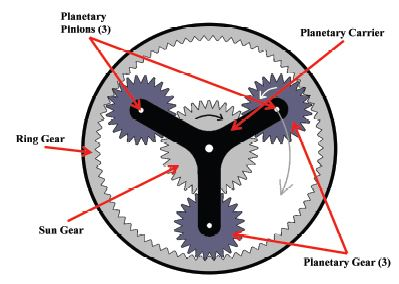
\includegraphics{PGB}
	\caption{Planetary Gearbox Layout\cite{gearbox}}
	\label{simulationfigure}
\end{figure}

The characters of planetary gearbox make it suitable for large transmission ratio, high load and split input or output circumstances. So it is widely used in wind turbines, lathes, automobiles and helicopters. The widely appliance and tough working environment of planetary gearbox require it to be highly dependable. Failures of planetary gearbox may lead to huge economic losses as well as safety incidents. But the compact and complex structure on the other hand make it difficult to monitor its condition. Especially when the load and operating speed are varying. This project focuses on the varying speed conditions.




\section{Planetary Gearbox fault diagnosis}

Vibration of gear is caused by the geometric deviation of gears and teeth deformation under load. These two effects introduce a 'meshing error' or 'transmission error' (TE). \cite{VBCM}The transmission error could be divided into three types: unloaded static TE, loaded static TE and dynamic TE. The unloaded static TE could be measured under a very light load, and it is realised to be caused by the geometric deviation. The load static TE is introduced by the tooth deflection under a constant load torque. Dynamic TE is caused by the fluctuation of torque and transmission speed.


\subsection{Vibration generated by gear}

Based on the understanding of transmission error, vibration generated by gears is classified as follows: \cite{VBCM}

1) Mean effects for all tooth pairs

The mean effects here are the same for all tooth pairs. Therefore dominated by harmonics of tooth-mesh frequencies. It could be sub divided into tree parts: 

	- Tooth deflection due to mean torque.
		
	- The mean part of initial profile errors resulting from manufacturing.	
	
	- Uniform wear over all teeth.

2) Variation from the mean.

Variation from the mean could give rise to side bands of harmonics and maybe caused by:

	- Slow variations, such as distortion and runout.	
	
	- Local faults, such as tooth spalls and root cracks.	
	
	- Random errors.	
	
	- Systematic erros.

Due to limitation of time and resource, the main fault investigated in this project is Local fault, including tooth spalls and root cracks.

1)	Normal operation

2)	Fault, spalls and cracks

\subsection{Diagnosis techniques}

1)	Standard Indicators

2)	wavelet

3)	Cepstrum

4)	TSA

5)	Order tracking

6)	Machine learning method


\section{Variable Speed}